% ==================================================================
% PSet 1 Report (Template-based)
% Based on: paper_summary.tex (Rafael template)
% ==================================================================
\documentclass[12pt]{article}

\newif\ifmyoption
\myoptiontrue

% --- Core settings & fonts ---
\usepackage[T1]{fontenc}
\usepackage[sc]{mathpazo}
\usepackage{geometry}
\geometry{top=1in, bottom=1in, left=1in, right=1in}

% --- Figures & floats ---
\usepackage{graphicx}
\usepackage{subfig}
\usepackage{float}
\usepackage[skip=.5em,font=normalsize,labelfont=bf]{caption}
\usepackage{pgfplots}
\usepgfplotslibrary{groupplots}
\pgfplotsset{compat=1.18}

% --- Utilities ---
\usepackage{url}
\usepackage{booktabs}
\usepackage{tabularx}
\usepackage{setspace}
\usepackage{csquotes}
\usepackage{derivative}
\usepackage{dirtytalk}

% --- Bibliography (kept for consistency; optional) ---
\usepackage[round]{natbib}
\setcitestyle{authoryear,round,semicolon,aysep={}}
\renewcommand\refname{References}

% --- Math ---
\usepackage{amsmath,amssymb,amsfonts,amsthm,mathtools}
\usepackage{bbm}
\usepackage{xparse}
\newcommand{\E}{\mathbb{E}}
\DeclareMathOperator*{\argmin}{arg\,min}
\DeclareMathOperator*{\argmax}{arg\,max}
\DeclareMathOperator{\Var}{Var}
\DeclareMathOperator{\Cov}{Cov}
\DeclareMathOperator{\Corr}{Corr}

% --- Lists & refs ---
\usepackage{enumitem}
\usepackage[colorlinks=true,linkcolor=blue,urlcolor=blue,citecolor=blue]{hyperref}
\usepackage{cleveref}

% --- Algorithms ---
\usepackage{algorithm}
\usepackage{algpseudocode}

\title{\textbf{Problem Set 1: Basic Numerical Tools}\\[0.2cm]\large Python Solutions}
\author{Rafael Lincoln}
\date{\today}

\begin{document}
\begin{titlepage}
\centering

\includegraphics[width=0.7\textwidth]{figures/New_York_University-Logo.wine}\par
\vspace{1cm}
{\LARGE\bfseries Problem Set 1\par}
\vspace{0.4cm}
{\large Python Solutions \par}
\vspace{1.2cm}
{\large Rafael Lincoln\par}
\vspace{0.1cm}
{\ttfamily rafael.lincoln@nyu.edu\par}
\vfill
{\large\textsc{New York University}\par}
\vspace{0.4cm}
{\large \today\par}
\end{titlepage}

\thispagestyle{empty}

\pagenumbering{roman}
\tableofcontents
\clearpage
\pagenumbering{arabic}
\setcounter{page}{1}

\begin{onehalfspacing}

\section{Solving Linear Equations and Interpolation}

\subsection{Vandermonde system}
We solve the linear system \(Ax=b\) where \(A\in\mathbb{R}^{n\times n}\) is a Vandermonde-type matrix with entries
\[
  A_{ij} = i^{\,n-j}, \qquad i,j\in\{1,\dots,n\},
\]
and \(b\in\mathbb{R}^{n}\) has entries
\[
  b_i = \sum_{k=0}^{n-1} i^k
  = \begin{cases}
  n, & i=1,\\
  \dfrac{i^n - 1}{i-1}, & i>1.
  \end{cases}
\]
The true solution is \(x=\mathbf{1}\). We report the conditioning of \(A\) and the numerical errors \(\lVert x-\mathbf{1}\rVert_2\) and \(\lVert Ax-b\rVert_2\) for \(n\in\{5,10,15\}\).

\begin{table}[H]
\centering
\caption{Vandermonde solve diagnostics}
\label{tab:pset1-vandermonde}
\begin{tabular}{rccc}
\toprule
\(n\) & \(\kappa_2(A)\) & \(\lVert x-\mathbf{1}\rVert_2\) & \(\lVert Ax-b\rVert_2\) \\
\midrule
5 & \(2.62\times 10^{4}\) & \(3.20\times 10^{-13}\) & \(1.14\times 10^{-13}\) \\
10 & \(2.11\times 10^{12}\) & \(7.89\times 10^{-7}\) & \(1.81\times 10^{-7}\) \\
15 & \(2.58\times 10^{21}\) & \(2.17\times 10^{2}\) & \(2.29\) \\
\bottomrule
\end{tabular}
\end{table}

\noindent where \(\kappa_2(A)\) is the condition number of \(A\) in the 2-norm, which is defined as:
\begin{align}
\kappa_2(A) = \|A\|_2 \|A^{-1}\|_2,
\end{align}
where $ \|A\|_2$ is the spectral norm of $A$, corresponding to the largest singular value of $A$. From Table~\ref{tab:pset1-vandermonde}, we see that the condition number grows rapidly as $n$ increases, indicating that the Vandermonde system is ill-conditioned. Hence, for $n$ values larger than 10, the solution is not accurate as columns become nearly linearly dependent in finite precision arithmetic.


\subsection{Polynomial interpolation of \(\log(s)\)}
We approximate \(f(s)=\log(s)\) on \(s\in[1,10]\) by a polynomial of degree \(n-1\),
\[
  \hat f_n(s)=x_1 + x_2 s + \dots + x_n s^{n-1}.
\]
We fit coefficients by (overdetermined) least squares using \(m=100\) equally-spaced points. For \(n\in\{5,10,15,20\}\) we plot the approximant on a fine grid and the approximation error \(\hat f_n(s)-\log(s)\), and we report the Euclidean norm of the error on the fine grid and the condition number of the regression matrix.

\begin{figure}[H]
\centering
\begin{tikzpicture}
\begin{groupplot}[
  group style={group size=2 by 1, horizontal sep=1.4cm},
  width=0.48\textwidth,
  height=0.34\textwidth,
  xlabel={$s$},
  legend style={font=\footnotesize, cells={anchor=west}},
]
\nextgroupplot[
  title={Polynomial approximations},
  ylabel={$f(s)$},
]
\addplot[black, thick] table[x=s,y=true,col sep=comma]{problem1_poly_approx.csv};
\addlegendentry{true}
\addplot[blue] table[x=s,y=pred5,col sep=comma]{problem1_poly_approx.csv};
\addlegendentry{$n=5$}
\addplot[red] table[x=s,y=pred10,col sep=comma]{problem1_poly_approx.csv};
\addlegendentry{$n=10$}
\addplot[green!50!black] table[x=s,y=pred15,col sep=comma]{problem1_poly_approx.csv};
\addlegendentry{$n=15$}
\addplot[purple] table[x=s,y=pred20,col sep=comma]{problem1_poly_approx.csv};
\addlegendentry{$n=20$}

\nextgroupplot[
  title={Approximation error},
  ylabel={$\hat f_n(s)-\log(s)$},
]
\addplot[black, thin] coordinates {(1,0) (10,0)};
\addplot[blue] table[x=s,y=err5,col sep=comma]{problem1_poly_approx.csv};
\addplot[red] table[x=s,y=err10,col sep=comma]{problem1_poly_approx.csv};
\addplot[green!50!black] table[x=s,y=err15,col sep=comma]{problem1_poly_approx.csv};
\addplot[purple] table[x=s,y=err20,col sep=comma]{problem1_poly_approx.csv};
\end{groupplot}
\end{tikzpicture}
\caption{Polynomial approximations of $\log(s)$ (left) and approximation errors (right) for degrees $n-1$ with $n\in\{5,10,15,20\}$, using a monomial basis and least squares on $m=100$ grid points.}
\label{fig:pset1-poly-approx}
\end{figure}
\vspace{1.5em}

\noindent The key numerical lesson from Problem 1.1 carries over directly to polynomial approximation: the least-squares design matrix has columns $1,s,s^2,\dots,s^{n-1}$, so it is \emph{Vandermonde-like} in the monomial basis. As $n$ grows, the columns become increasingly ill-conditioned (similar to Table~\ref{tab:pset1-vandermonde}), so the fitted coefficients can become extremely sensitive to rounding error and to small perturbations in the data. Therefore, increasing $n$ does not guarantee a uniformly better approximation: the function space is richer, but numerical instability can dominate and produce oscillatory or distorted fits (often most visible near the boundaries of $[1,10]$) and non-monotone error behavior.




\clearpage
\section{Optimal Labor Supply}


We consider a static equilibrium with heterogeneous ability. There is a continuum of households indexed by ability $e \in [1,\bar{e}]$, distributed according to a truncated Pareto distribution $e \sim \widehat{F}(e)$. Each household chooses hours $h \ge 0$ to maximize CRRA utility separable in labor and consumption, subject to a budget constraint. Production is Cobb--Douglas in aggregate labor, with decreasing returns to scale, and the government levies a linear tax on labor income and rebates revenue lump-sum.

The goal is to compute the equilibrium allocation: a wage $W$, a lump-sum transfer $T$, and a schedule of hours $h(e)$ and consumption $c(e)$ such that (i) households optimize, (ii) firms maximize profits, and (iii) the goods market clears.

\subsection{Setup}

Ability is distributed with truncated Pareto cdf $\widehat{F}(e) = (1 - e^{-\alpha}) / (1 - \bar{e}^{-\alpha})$ on $[1,\bar{e}]$. We discretize this distribution using Gauss--Legendre quadrature: nodes $\{e_i\}_{i=1}^n$ and weights $\{\omega_i\}_{i=1}^n$ with $\sum_i \omega_i = 1$, so that expectations are approximated by $\E[g(e)] \approx \sum_i \omega_i g(e_i)$. Aggregate labor supply is
\begin{equation}
  L = \sum_{i=1}^n \omega_i e_i h_i.
\end{equation}
Output is $Y = L^\eta$ with $\eta \in (0,1)$. Under perfect competition, the wage is
\begin{equation}
  W = \eta L^{\eta - 1}.
\end{equation}
Tax revenue is rebated lump-sum; with tax rate $\tau$ on labor income, the transfer is
\begin{equation}
  T = L^\eta - (1-\tau) W L.
\end{equation}
Household $i$ has consumption
\begin{equation}
  c_i = T + (1-\tau) W e_i h_i.
\end{equation}
With CRRA utility in consumption and disutility of labor, the first-order condition for interior $h_i > 0$ is
\begin{equation}
  h_i^\gamma = (1-\tau) W e_i c_i^{-\sigma}.
\end{equation}

\subsubsection{System of equations}

Collect the vector of hours $\mathbf{h} = (h_1,\ldots,h_n)^\top$. Define aggregate objects as functions of $\mathbf{h}$:
\begin{align}
\begin{split}
  L(\mathbf{h}) &= \sum_{i=1}^n \omega_i e_i h_i, \\
  W(\mathbf{h}) &= \eta L(\mathbf{h})^{\eta-1}, \\
  T(\mathbf{h}) &= L(\mathbf{h})^\eta - (1-\tau) W(\mathbf{h}) L(\mathbf{h}).
\end{split}
\end{align}
Consumption of household $i$ is $c_i(\mathbf{h}) = T(\mathbf{h}) + (1-\tau) W(\mathbf{h}) e_i h_i$. The residual for the FOC of household $i$ is
\begin{equation}
  F_i(\mathbf{h}) = h_i^\gamma - (1-\tau) W(\mathbf{h}) e_i c_i(\mathbf{h})^{-\sigma}.
\end{equation}
Equilibrium is a root of the $n$-dimensional system
\begin{equation}
  \mathbf{F}(\mathbf{h}) = \mathbf{0}.
\end{equation}
Goods market clearing is implied: $\sum_i \omega_i c_i = Y = L^\eta$ at a solution.

\subsection{Solution methods}

We implement two approaches: (1) solve $\mathbf{F}(\mathbf{h})=\mathbf{0}$ in one shot with a robust Broyden method; (2) solve by fixed point on the wage $W$, with an inner Broyden step for the vector of hours given $W$.

\subsubsection{Approach 1: Full system (Broyden on $\mathbf{F}$)}

We solve the coupled system $\mathbf{F}(\mathbf{h})=\mathbf{0}$ directly. Because the Jacobian of $\mathbf{F}$ is dense and the system can be ill-scaled, we use the CompEcon-style Broyden method (inverse Jacobian approximation, backstepping line search, restarts), i.e.\ \texttt{broyden(..., method='compecon')}.

\begin{algorithm}[H]
\caption{Full-system Broyden for labor supply equilibrium}
\label{alg:broyden-full}
\begin{algorithmic}[1]
\State \textbf{Input:} Residual $\mathbf{F}$, initial guess $\mathbf{h}^{(0)}$, tolerance $\varepsilon$, max iterations $K$
\State \textbf{Output:} Equilibrium hours $\mathbf{h}^*$
\State $k \gets 0$
\While{$k < K$ and $\|\mathbf{F}(\mathbf{h}^{(k)})\|_\infty > \varepsilon$}
  \State Update $\mathbf{h}^{(k+1)}$ via Broyden (inverse Jacobian + line search)
  \State $k \gets k + 1$
\EndWhile
\State \textbf{return} $\mathbf{h}^{(k)}$
\end{algorithmic}
\end{algorithm}

\subsubsection{Approach 2: Fixed point on wages (inner componentwise Broyden)}

Given a guess for the wage $W$, the transfer is $T = L^\eta - (1-\tau) W L$ with $L = \sum_i \omega_i e_i h_i$. For fixed $W$ and $T$, each household's FOC is a scalar equation in $h_i$ with bounds $0 \le h_i \le \bar{h}$. We solve this vectorized system with safeguarded componentwise Broyden, i.e.\ \texttt{broyden(..., method='componentwise', a=0, b=}$\bar{h}$\texttt{)}. Then we aggregate $L$, update $W \leftarrow \eta L^{\eta-1}$ (optionally damped), and repeat until $W$ converges.

\begin{algorithm}[H]
\caption{Wage fixed-point with inner componentwise Broyden}
\label{alg:wage-fp}
\begin{algorithmic}[1]
\State \textbf{Input:} Parameters $(\tau,\eta,\sigma,\gamma)$, quadrature $(e_i,\omega_i)$, bounds $(\underline{h},\bar{h})$, tolerance $\varepsilon$, max outer iterations $K_{\mathrm{out}}$, max inner iterations $K_{\mathrm{in}}$
\State \textbf{Output:} Equilibrium wage $W^*$ and hours $\mathbf{h}^*$
\State $W \gets W^{(0)}$ (e.g.\ initial guess)
\State $\mathbf{h} \gets \mathbf{h}^{(0)}$ (e.g.\ $\mathbf{1}$)
\For{$k = 1$ to $K_{\mathrm{out}}$}
  \State $L \gets \sum_i \omega_i e_i h_i$; \; $T \gets L^\eta - (1-\tau) W L$
  \State Solve for $\mathbf{h}$: FOC residuals in $h_i$ given $(W,T)$ equal zero, with $a_i = \underline{h}$, $b_i = \bar{h}$, using componentwise Broyden (max $K_{\mathrm{in}}$ iterations)
  \State $L_{\mathrm{new}} \gets \sum_i \omega_i e_i h_i$; \; $W_{\mathrm{new}} \gets \eta L_{\mathrm{new}}^{\eta-1}$
  \If{$|W_{\mathrm{new}} - W| < \varepsilon$}
    \State \textbf{return} $W_{\mathrm{new}}$, $\mathbf{h}$
  \EndIf
  \State $W \gets W + \lambda (W_{\mathrm{new}} - W)$ (damping $\lambda \in (0,1]$ optional)
\EndFor
\State \textbf{return} $W$, $\mathbf{h}$
\end{algorithmic}
\end{algorithm}

\begin{figure}[H]
\centering
\subfloat[Broyden iteration trace]{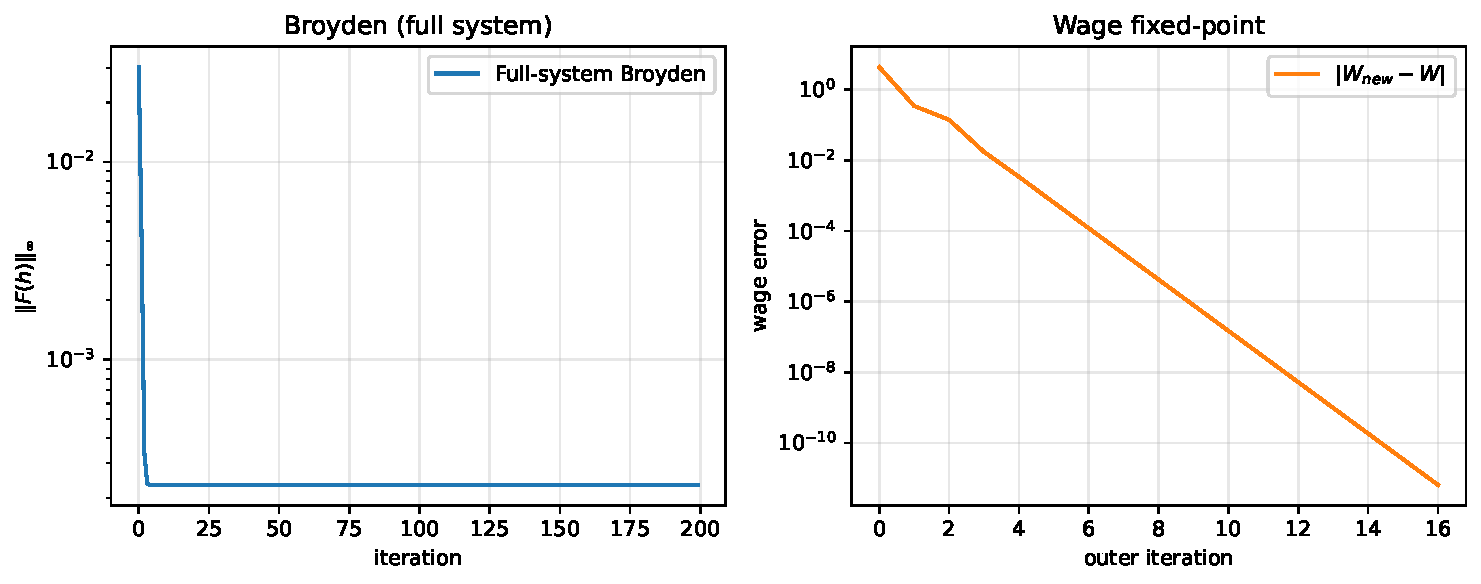
\includegraphics[width=0.48\textwidth]{figures/problem2_broyden_trace}}
\hfill
\subfloat[Equilibrium labor curve]{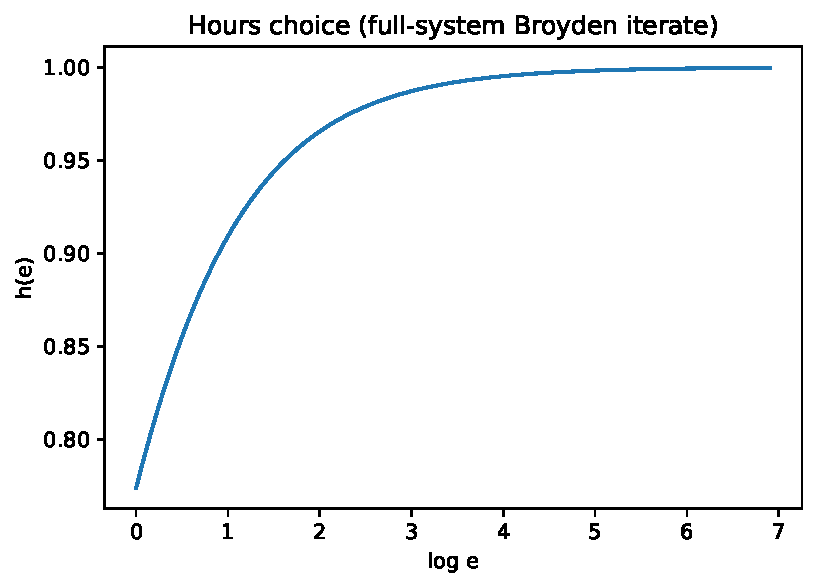
\includegraphics[width=0.48\textwidth]{figures/problem2_labor_curve}}
\caption{Broyden convergence (Approach 1: full-system CompEcon-style) and equilibrium hours $h(e)$ vs.\ $\log e$.}
\label{fig:problem2-results}
\end{figure}

\subsection{Implementation notes}

\begin{itemize}[leftmargin=*]
  \item \textbf{Quadrature (Sec.\ 2.1):} We use Gauss--Legendre nodes and weights on $[1,\bar{e}]$ and multiply weights by the truncated Pareto pdf so that $\sum_i \omega_i = 1$. We check that the first three moments match the analytical formulas.
  \item \textbf{Approach 1:} We call \texttt{broyden(..., method='compecon')} with guardrails in the residual (clip $h$ to $[10^{-12},\bar{h}]$, penalize $c \le 0$) to avoid numerical explosions.
  \item \textbf{Approach 2:} We call \texttt{broyden(..., method='componentwise', a=hmin, b=hmax)} for the inner FOC system given $(W,T)$. The outer loop updates $W$ until $|W_{\mathrm{new}} - W| < \varepsilon$.
  \item \textbf{Checks:} We verify goods market clearing $\sum_i \omega_i c_i = L^\eta$ and report the FOC residual norm and transfer $T$, labor $L$, output $Y$, and wage $W$.
\end{itemize}

% \subsection*{Pause / check}
% \begin{itemize}[leftmargin=*]
%   \item Check quadrature weights sum to 1 and moments match formulas.
%   \item Check goods market: $\sum_i \omega_i c_i = L^\eta$.
% \end{itemize}
\clearpage
\section{Calibration by Simulation}


We consider an economy with a continuum of firms indexed by $i$. Each firm $i$ has idiosyncratic productivity $z_{it}$ and chooses labor demand $\ell_{it} \ge 0$. Output is produced with a Cobb-Douglas technology in productivity and labor:
\begin{equation}
  y_{it} = (z_{it})^{1-\eta}\, (\ell_{it})^{\eta},
\end{equation}
where $\eta \in (0,1)$. In a partial equilibrium setting we normalize the wage $W = 1$. The firm's problem is
\begin{equation}
  \max_{\ell_{it} \ge 0} \quad y_{it} - W \ell_{it} = (z_{it})^{1-\eta}\, (\ell_{it})^{\eta} - \ell_{it}.
\end{equation}
The first-order condition $\eta\, (z_{it})^{1-\eta}\, (\ell_{it})^{\eta-1} = 1$ yields optimal labor
\begin{equation}
  \ell_{it} = \eta^{1/(1-\eta)}\, z_{it},
\end{equation}
and therefore output
\begin{equation}
  y_{it} = (z_{it})^{1-\eta}\, \bigl(\eta^{1/(1-\eta)}\, z_{it}\bigr)^{\eta}
  = \eta^{\eta/(1-\eta)}\, z_{it}.
\end{equation}
Hence $\log y_{it} = \log z_{it} + \text{const}$: (log) output and (log) productivity coincide up to a constant. We observe a panel of log productivity (or log output) and seek to calibrate the parameters of the stochastic process that governs $\log z_{it}$ by matching selected moments.

\subsection{Stochastic process for log productivity}

We drop the firm index $i$ when describing the law of motion. Let $y_t \equiv \log z_{it}$ denote log productivity (or log output) and $x_t \equiv \log \hat z_{it}$ the persistent component. The process is
\begin{align*}
  y_t &= x_t + \varepsilon_t, \qquad \varepsilon_t \stackrel{\text{iid}}{\sim} \mathcal{N}(0,\sigma_\varepsilon^2), \\
  x_t &= \rho x_{t-1} + u_t, \qquad u_t \stackrel{\text{iid}}{\sim} \mathcal{N}(0,\sigma_u^2), \qquad |\rho| < 1, \\
  u_t &\perp \varepsilon_s \quad \forall t,s.
\end{align*}
So log productivity is the sum of a persistent AR(1) component $x_t$ and an iid transitory shock $\varepsilon_t$.

\subsection{Analytical moments}

\subsubsection{Variance and standard deviation of $\log y_t$}

The persistent component has stationary variance $\Var(x_t) = \sigma_u^2/(1-\rho^2)$. Hence
\begin{align*}
  \Var(y_t) &= \Var(x_t) + \Var(\varepsilon_t)
  = \frac{\sigma_u^2}{1-\rho^2} + \sigma_\varepsilon^2, \\
  \operatorname{sd}(y_t) &= \sqrt{\frac{\sigma_u^2}{1-\rho^2} + \sigma_\varepsilon^2}.
\end{align*}

\subsubsection{Variance and standard deviation of $\Delta y_t \equiv y_t - y_{t-1}$}

Using $\Var(\Delta y_t) = 2\Var(y_t) - 2\Cov(y_t,y_{t-1})$ and $\Cov(y_t,y_{t-1}) = \Cov(x_t,x_{t-1}) = \rho \Var(x_t) = \rho \sigma_u^2/(1-\rho^2)$,
\begin{align*}
  \Var(\Delta y_t)
  &= 2\left(\frac{\sigma_u^2}{1-\rho^2}+\sigma_\varepsilon^2\right)
  - 2\,\rho\,\frac{\sigma_u^2}{1-\rho^2}
  = 2\left(\frac{\sigma_u^2}{1+\rho}+\sigma_\varepsilon^2\right), \\
  \operatorname{sd}(\Delta y_t) &= \sqrt{2\left(\frac{\sigma_u^2}{1+\rho}+\sigma_\varepsilon^2\right)}.
\end{align*}

\subsubsection{Autocorrelations of $\log y_t$}

For $k \ge 1$,
\begin{align*}
  \Cov(y_t,y_{t-k})
  &= \Cov(x_t,x_{t-k})
  = \rho^k \Var(x_t)
  = \rho^k \,\frac{\sigma_u^2}{1-\rho^2}, \\
  \Corr(y_t,y_{t-k})
  &= \frac{\Cov(y_t,y_{t-k})}{\Var(y_t)}
  = \rho^k \cdot \frac{\frac{\sigma_u^2}{1-\rho^2}}{\frac{\sigma_u^2}{1-\rho^2}+\sigma_\varepsilon^2}.
\end{align*}
We target the autocorrelations at lags $k=1$, $3$, and $5$:
\begin{align*}
  \Corr(y_t,y_{t-1}) &= \rho \cdot \frac{\frac{\sigma_u^2}{1-\rho^2}}{\frac{\sigma_u^2}{1-\rho^2}+\sigma_\varepsilon^2}, \\
  \Corr(y_t,y_{t-3}) &= \rho^3 \cdot \frac{\frac{\sigma_u^2}{1-\rho^2}}{\frac{\sigma_u^2}{1-\rho^2}+\sigma_\varepsilon^2}, \\
  \Corr(y_t,y_{t-5}) &= \rho^5 \cdot \frac{\frac{\sigma_u^2}{1-\rho^2}}{\frac{\sigma_u^2}{1-\rho^2}+\sigma_\varepsilon^2}.
\end{align*}

\subsection{Simulation and target moments}

We simulate a panel of $N = 100{,}000$ firms over $T = 10$ periods. For each firm we draw the initial persistent component from the ergodic distribution $\mathcal{N}(0,\sigma_u^2/(1-\rho^2))$, then evolve $x_t$ and add iid $\varepsilon_t$ to obtain $y_t = x_t + \varepsilon_t$. From the simulated panel we compute:
\begin{itemize}[leftmargin=*]
  \item standard deviation of $\log y_t$,
  \item standard deviation of the one-year change $\Delta y_t = y_t - y_{t-1}$,
  \item autocorrelations of $y_t$ at lags 1, 3, and 5.
\end{itemize}
We match these to the following target moments (from the data): $\operatorname{sd}(y) = 1.31$, $\operatorname{sd}(\Delta y) = 0.59$, $\Corr(y_t,y_{t-1}) = 0.90$, $\Corr(y_t,y_{t-3}) = 0.87$, $\Corr(y_t,y_{t-5}) = 0.85$.

\Cref{fig:problem3-dlogz} shows the distribution of log-productivity changes at horizons 1, 3, and 5 years from the simulated panel (using initial parameter guesses). Under this two-component process, the change $\Delta_k y_t = y_t - y_{t-k}$ is the sum of two independent normal random variables and is therefore normal; the empirical densities align with this.

\begin{figure}[H]
  \centering
  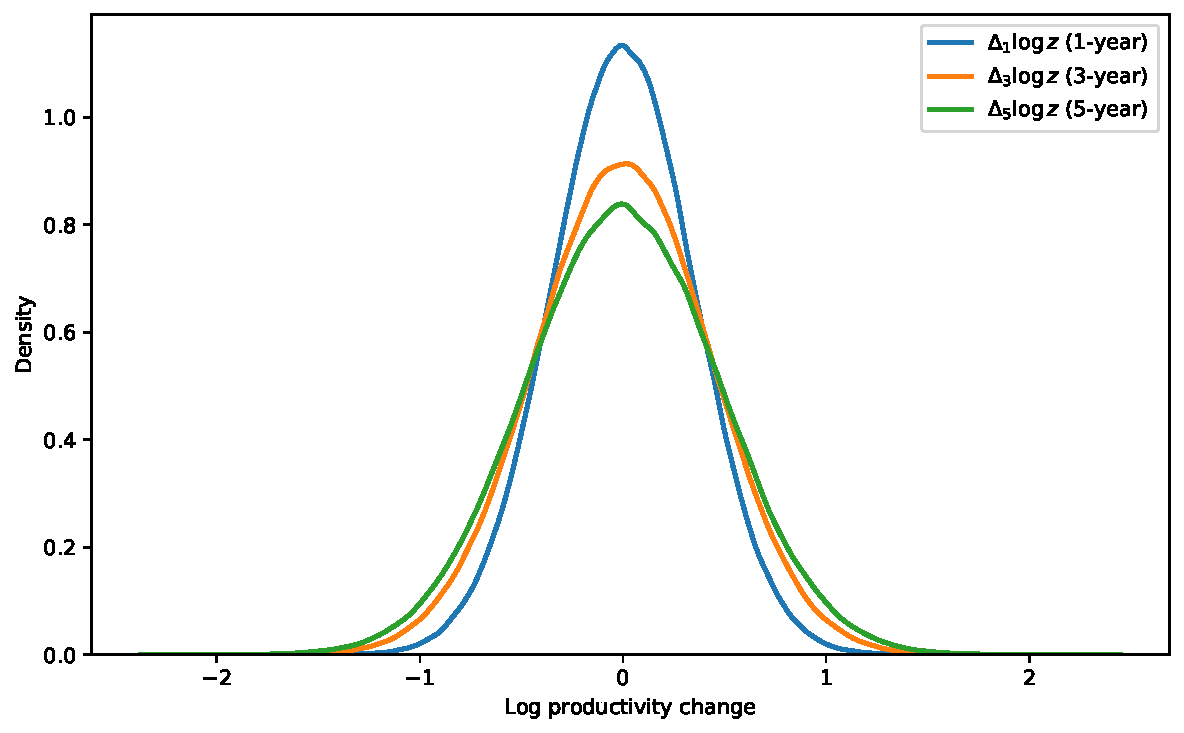
\includegraphics[width=0.75\textwidth]{figures/problem3_dlogz}
  \caption{Distribution of log-productivity changes: density of $\Delta_1 \log z$, $\Delta_3 \log z$, and $\Delta_5 \log z$ from the simulated panel (KDE).}
  \label{fig:problem3-dlogz}
\end{figure}

\subsection{Estimation: Nelder-Mead}

We estimate $\theta = (\rho,\sigma_u,\sigma_\varepsilon)$ by minimizing the sum of squared errors between the five model moments and the five target moments (SSE). We use the Nelder-Mead simplex algorithm (no derivatives), with simple bounds: $\rho \in [0.70, 0.99]$, $\sigma_u,\sigma_\varepsilon \in [0.01, 0.50]$. At each iteration we simulate the panel once (fixed seed for reproducibility) and compute the moments; the objective is the squared Euclidean norm of the moment residual vector.

\Cref{fig:problem3-nelder} plots the SSE at each Nelder-Mead iteration. The algorithm converges to a low SSE, and the resulting parameter vector reproduces the target moments closely (e.g.\ $\hat\rho \approx 0.986$, $\hat\sigma_u \approx 0.21$, $\hat\sigma_\varepsilon \approx 0.39$).

\begin{figure}[H]
  \centering
  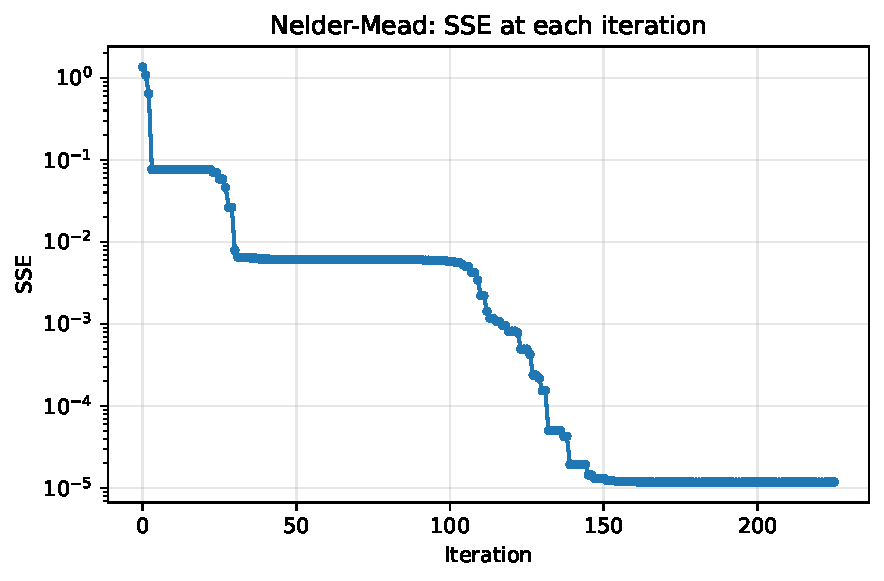
\includegraphics[width=0.65\textwidth]{figures/problem3_nelder_sse}
  \caption{Nelder-Mead: SSE (sum of squared moment errors) at each iteration.}
  \label{fig:problem3-nelder}
\end{figure}

\subsection{Implementation notes}

\begin{itemize}[leftmargin=*]
  \item \textbf{Simulation:} Initial $x_0$ is drawn from $\mathcal{N}(0,\sigma_u^2/(1-\rho^2))$; then $x_t = \rho x_{t-1} + u_t$ and $y_t = x_t + \varepsilon_t$ for $t=1,\ldots,T-1$.
  \item \textbf{Moments:} Standard deviations and correlations are computed from the flattened panel (all firms and time periods used for each moment).
  \item \textbf{Nelder-Mead:} We use \texttt{hetmacro.optimize.nelder\_mead} with \texttt{return\_info=True} to record the objective value at each iteration for the convergence plot.
\end{itemize}

\subsection{Extension: Jump-diffusion (fat tails)}

To capture fat tails and leptokurtic distributions in the data, we extend the persistent component to a \emph{jump-diffusion}. Idiosyncratic log productivity is $\tilde{y}_{it} = x_{it} + \varepsilon_{it}$ with $\varepsilon_{it} \sim \mathcal{N}(0,\sigma_\varepsilon^2)$. The persistent state follows
\begin{align*}
  x_{it} &= \rho x_{i,t-1} + \eta_{it} + J_{it}, \qquad \eta_{it} \stackrel{\text{iid}}{\sim} \mathcal{N}(0,\sigma_\eta^2), \\
  J_{it} &= b_{it}\, \kappa_{it}, \qquad b_{it} \sim \text{Bernoulli}(\pi), \quad \kappa_{it} \sim \mathcal{N}(\mu_J,\sigma_J^2),
\end{align*}
with $\varepsilon_{it}$, $\eta_{it}$, $b_{it}$, $\kappa_{it}$ mutually independent. The jump term delivers occasional large moves in $\Delta \tilde{y}_{it}$, generating fat tails while preserving the AR(1)+noise structure. The stationary variance of $x$ is $\Var(x) = (\sigma_\eta^2 + \Var(J))/(1-\rho^2)$ with $\Var(J) = \pi\sigma_J^2 + \pi(1-\pi)\mu_J^2$; we draw $x_0$ from $\mathcal{N}(0,\sqrt{\Var(x)})$.

We estimate $\theta = (\rho,\sigma_\eta,\sigma_\varepsilon,\pi,\mu_J,\sigma_J)$ by minimizing the same SSE over the same five target moments (simulation-based; no closed-form moments for the jump model). Bounds: $\rho \in [0.70, 0.99]$, $\sigma_\eta,\sigma_\varepsilon \in [0.01, 0.50]$, $\pi \in [0.01, 0.5]$, $\mu_J \in [-1, 1]$, $\sigma_J \in [0.01, 1]$. \Cref{fig:problem3-nelder-jump} shows the Nelder-Mead SSE trace for the 6-parameter problem; \Cref{fig:problem3-dlogz-jump} shows the distribution of log-productivity changes under the jump-diffusion fit, with fatter tails than the baseline.

\begin{figure}[H]
  \centering
  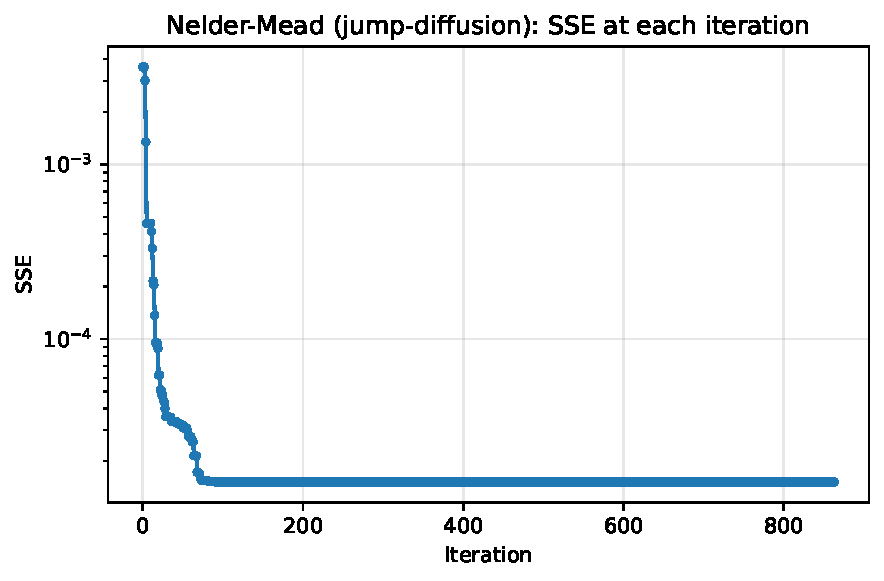
\includegraphics[width=0.65\textwidth]{figures/problem3_nelder_sse_jump}
  \caption{Nelder-Mead (jump-diffusion): SSE at each iteration.}
  \label{fig:problem3-nelder-jump}
\end{figure}

\begin{figure}[H]
  \centering
  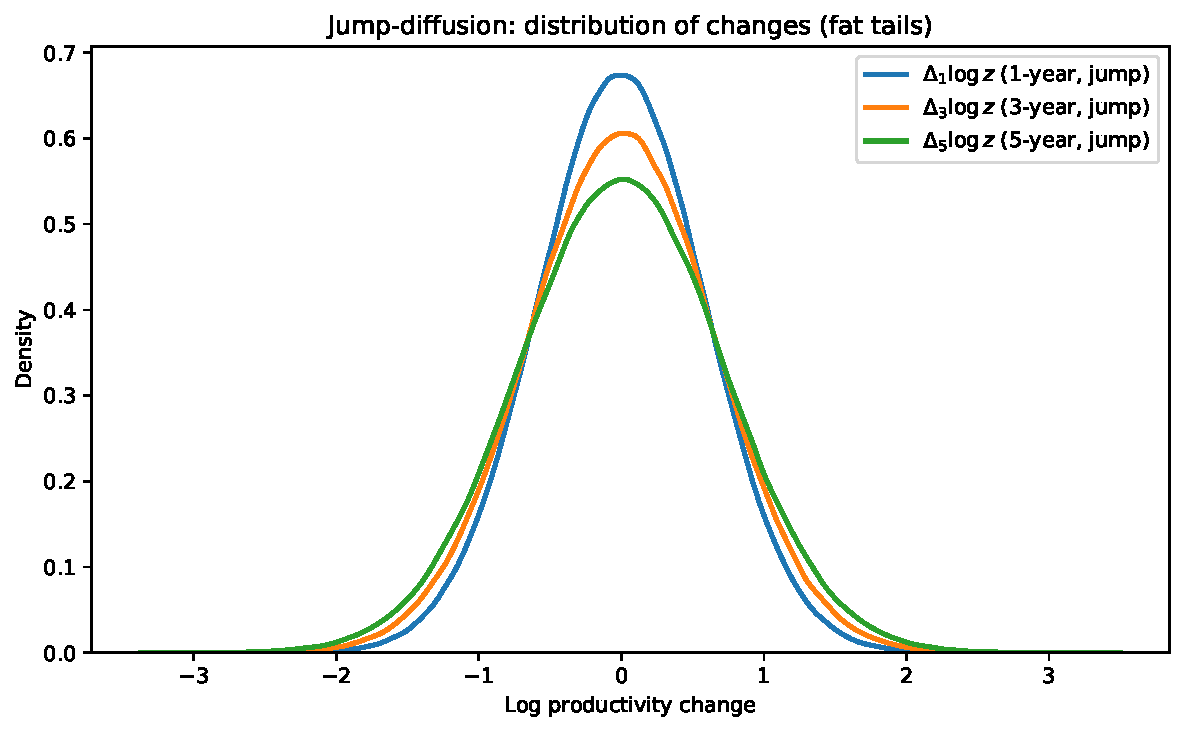
\includegraphics[width=0.75\textwidth]{figures/problem3_dlogz_jump}
  \caption{Jump-diffusion: distribution of log-productivity changes (fat tails).}
  \label{fig:problem3-dlogz-jump}
\end{figure}

\Cref{tab:problem3-moments} reports target vs.\ model moments for both specifications; \Cref{tab:problem3-parameters} reports the calibrated parameters. Tables are generated by \texttt{gen\_problem3\_figures.py}.

\begin{table}[H]
\centering
\caption{Target vs.\ model moments}
\label{tab:problem3-moments}
\begin{tabular}{lccc}
\toprule
Moment & Target & Baseline (AR(1)+noise) & Jump-diffusion \\
\midrule
$\operatorname{sd}(\log y)$ & 1.310 & 1.310 & 1.310 \\
$\operatorname{sd}(\Delta \log y)$ & 0.590 & 0.590 & 0.590 \\
$\Corr(y_t, y_{t-1})$ & 0.900 & 0.899 & 0.899 \\
$\Corr(y_t, y_{t-3})$ & 0.870 & 0.873 & 0.873 \\
$\Corr(y_t, y_{t-5})$ & 0.850 & 0.849 & 0.848 \\
\bottomrule
\end{tabular}
\end{table}

\begin{table}[H]
\centering
\caption{Calibrated parameters}
\label{tab:problem3-parameters}
\begin{tabular}{llc}
\toprule
Parameter & Model & Estimate \\
\midrule
$\rho$ & Baseline & 0.986 \\
$\sigma_u$ & Baseline & 0.210 \\
$\sigma_\varepsilon$ & Baseline & 0.390 \\
\midrule
$\rho$ & Jump-diffusion & 0.986 \\
$\sigma_\eta$ & Jump-diffusion & 0.198 \\
$\sigma_\varepsilon$ & Jump-diffusion & 0.390 \\
$\pi$ & Jump-diffusion & 0.050 \\
$\mu_J$ & Jump-diffusion & 0.000 \\
$\sigma_J$ & Jump-diffusion & 0.314 \\
\bottomrule
\end{tabular}
\end{table}


\clearpage
\section{Two-Period Labor Supply}


A consumer lives for two periods with preferences
\begin{equation}
  V = \sum_{t=1}^2 \beta^{t-1} \left( \frac{c_t^{1-\sigma}}{1-\sigma} - \frac{h_t^{1+\gamma}}{1+\gamma} \right),
\end{equation}
where $\sigma$ is the inverse elasticity of intertemporal substitution and $\gamma$ is the inverse Frisch elasticity of labor supply. The consumer saves in a riskless asset with interest rate $r$ and receives income $T + (1-\tau) W e_t h_t$ in period $t$. The budget constraints are
\begin{align}
  c_1 + a_2 &= T + (1-\tau) W e_1 h_1, \\
  c_2 &= T + (1-\tau) W e_2 h_2 + (1+r) a_2.
\end{align}
Efficiency is normalized to $e_1 = 1$ in the first period and equals $e_2$ in the second; we solve for different values of $e_2$. The consumer cannot borrow:
\begin{equation}
  a_2 \ge 0.
\end{equation}

\paragraph{Parameters.}
We use $\beta = 0.90$, $\sigma = 1.5$, $\gamma = 2$, $r = 0.04$, $W = 1$, $\tau = 0.25$, $T = 0.15$.

\subsection{Backward induction and optimality conditions}

The problem is solved by backward induction, respecting the no-borrowing constraint. In period 2, the consumer enters with assets $a$ and chooses $(c_2, h_2)$ subject to the budget constraint and the labor-leisure first-order condition. In period 1, the consumer chooses $(c_1, h_1)$ (and hence $a_2$) to maximize lifetime utility, subject to $a_2 \ge 0$.

\paragraph{Period 2.}
The labor-leisure FOC is
\begin{equation}
  h_2^\gamma = (1-\tau) W e_2\, c_2^{-\sigma}.
\end{equation}
With $c_2 = T + (1-\tau) W e_2 h_2 + (1+r) a$, substituting the budget into the FOC yields a single equation in $c_2$. Equivalently, define next-period assets as a function of current consumption and (implied) hours:
\begin{equation}
  a' = T + (1-\tau) W e h + (1+r) a - c.
\end{equation}
Given $c$, hours are backed out from the FOC: $h = \bigl( (1-\tau) W e\, c^{-\sigma} \bigr)^{1/\gamma}$. At the end of life we require $a_3 = 0$, so we solve for $c_2$ such that $a'(c_2) = 0$. This yields $c_2(a,e_2)$, $h_2(a,e_2)$, and the period-2 value
\begin{equation}
  V_2(a,e_2) = \frac{c_2(a,e_2)^{1-\sigma}}{1-\sigma} - \frac{h_2(a,e_2)^{1+\gamma}}{1+\gamma}.
\end{equation}

\paragraph{Period 1.}
For any $c_1$, hours satisfy $h_1^\gamma = (1-\tau) W e_1 c_1^{-\sigma}$ (with $e_1=1$) and savings are
\begin{equation}
  a_2 = T + (1-\tau) W e_1 h_1 - c_1.
\end{equation}
The upper bound $\bar{c}_1$ such that $a_2(\bar{c}_1) = 0$ ensures the no-borrowing constraint when we restrict $c_1 \in (0, \bar{c}_1]$. The consumer solves
\begin{equation}
  \max_{c_1 \in (0,\bar{c}_1]} \quad \frac{c_1^{1-\sigma}}{1-\sigma} - \frac{h_1^{1+\gamma}}{1+\gamma} + \beta V_2(a_2, e_2).
\end{equation}
At an interior optimum the Euler equation holds: $c_1^{-\sigma} = \beta(1+r) c_2^{-\sigma}$.

\subsection{Numerical solution: period 2}

We implement the period-2 solution as follows. For each pair $(a, e_2)$ on a grid, we find $c_2$ such that $a'(c_2) = 0$ using a bisection root-finder on the function \texttt{savings}$(c, a, e_2, p)$, which returns $a'$ given consumption (and implied hours from the labor FOC). This yields $c_2(a,e_2)$, $h_2(a,e_2)$, and $V_2(a,e_2)$.

\begin{algorithm}[H]
\caption{Period-2 solution (for each $(a,e_2)$)}
\label{alg:problem4-period2}
\begin{algorithmic}[1]
\State \textbf{Input:} Asset grid $a$, productivity $e_2$, parameters $p$
\State \textbf{Output:} $c_2(a,e_2)$, $h_2(a,e_2)$, $V_2(a,e_2)$
\For{each $(a_i, e_2)$}
  \State Bracket $c \in (0, \overline{\text{coh}})$ so that \texttt{savings}$(c,a_i,e_2,p)$ has a root
  \State $c_2 \gets \texttt{bisect}(\texttt{savings}, \ell, u; a_i, e_2, p)$ so that $a' = 0$
  \State $h_2 \gets$ hours from labor FOC given $c_2$
  \State $V_2 \gets u(c_2,h_2)$
\EndFor
\State \textbf{return} $V_2$, $c_2$, $h_2$
\end{algorithmic}
\end{algorithm}

\Cref{fig:problem4-period2} shows the period-2 consumption, hours, and value as surfaces over $(a, e_2)$.

\begin{figure}[H]
\centering
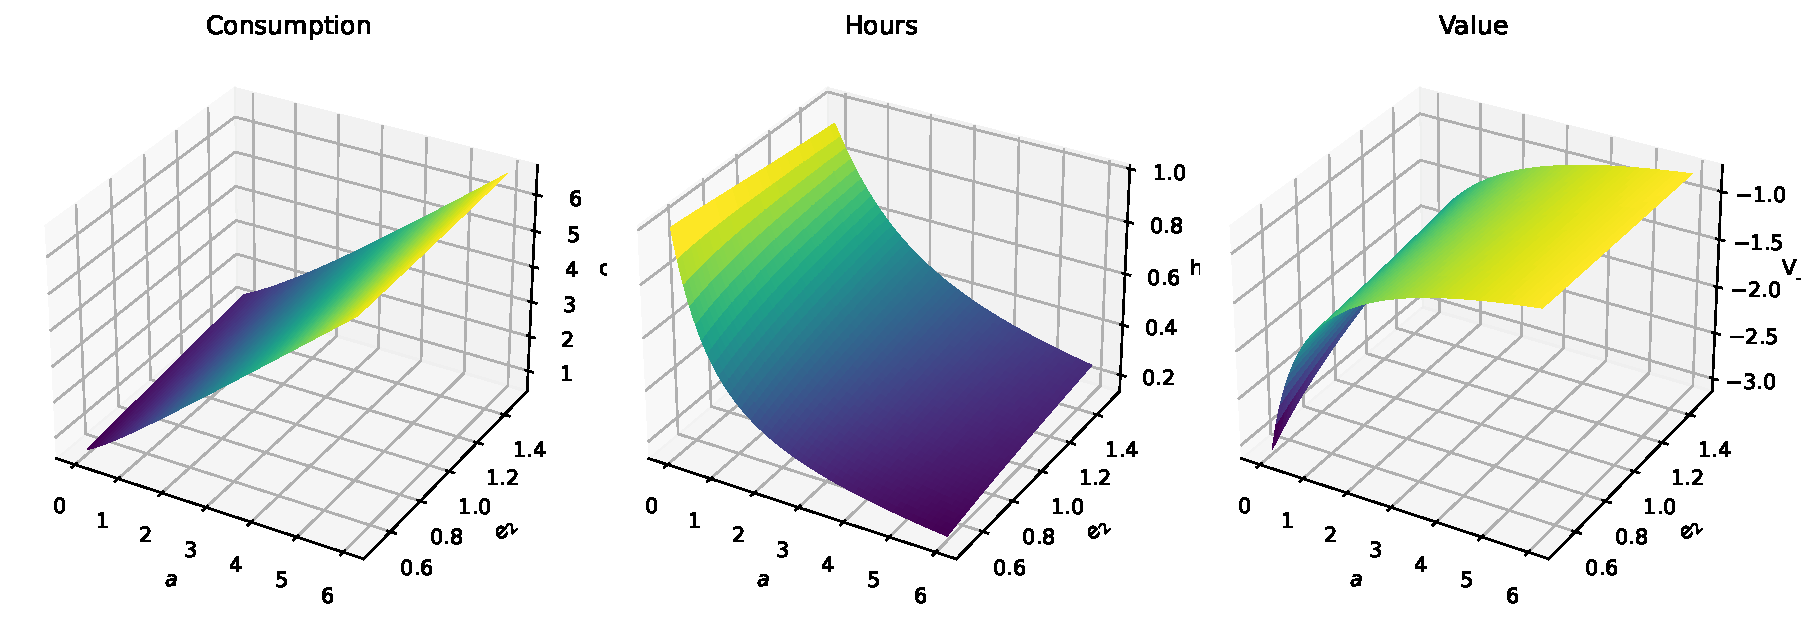
\includegraphics[width=\textwidth]{figures/problem4_period2_surfaces}
\caption{Period-2 policy and value: $c_2(a,e_2)$, $h_2(a,e_2)$, and $V_2(a,e_2)$ on a grid of assets $a$ and second-period productivity $e_2$.}
\label{fig:problem4-period2}
\end{figure}

\subsection{Numerical solution: period 1}

Given the period-2 value and policies, we solve the period-1 problem for each $e_2$ in a grid. Step (A): find the maximum feasible period-1 consumption $\bar{c}_1$ such that $a_2 = 0$ (bisection on \texttt{savings}$(c, 0, 1, p)$ with $a_1=0$, $e_1=1$). Step (B): maximize the period-1 lifetime value over $c_1 \in (0, \bar{c}_1]$ using golden-section search on the function that returns $u(c_1,h_1) + \beta V_2(a_2, e_2)$. Step (C): from the optimal $c_1$ we recover $h_1$, $a_2$, and then $c_2$, $h_2$ from the period-2 solution at $(a_2, e_2)$.

\begin{algorithm}[H]
\caption{Period-1 solution (for each $e_2$)}
\label{alg:problem4-period1}
\begin{algorithmic}[1]
\State \textbf{Input:} Productivity grid $e_2$, parameters $p$
\State \textbf{Output:} $c_1(e_2)$, $h_1(e_2)$, $a_2(e_2)$, $c_2(e_2)$, $h_2(e_2)$
\For{each $e_2$}
  \State $\bar{c}_1 \gets \texttt{bisect}(\texttt{savings}, \ell, u; 0, 1, p)$ so that $a_2 = 0$
  \State $c_1^* \gets \argmax_{c_1 \in (0,\bar{c}_1]} \bigl\{ u(c_1,h_1) + \beta V_2(a_2,e_2) \bigr\}$ via \texttt{golden\_search} on minus the objective
  \State $h_1 \gets$ hours from labor FOC; $a_2 \gets$ \texttt{savings}$(c_1^*, 0, 1, p)$
  \State $(c_2, h_2) \gets$ period-2 solution at $(a_2, e_2)$
\EndFor
\State \textbf{return} $c_1$, $h_1$, $a_2$, $c_2$, $h_2$
\end{algorithmic}
\end{algorithm}

The policy functions we report are expressed as functions of $e_2$ only. This is because we condition on the asset choice $a_2$ being the one chosen optimally in period 1 given $e_2$ (and $a_1=0$). So for each $e_2$, the plotted $c_1$, $h_1$, $a_2$, $c_2$, $h_2$ are the equilibrium choices along that path; they are not the full policy functions $c_2(a,e_2)$ and $h_2(a,e_2)$ over all $a$, but the realized consumption and hours given the endogenous $a_2(e_2)$.

We plot consumption, hours, and assets only for \emph{interior} points where $a_2 > 0$ (non-binding borrowing constraint), so that the Euler equation is approximately satisfied and the curves are smooth.

\begin{figure}[H]
\centering
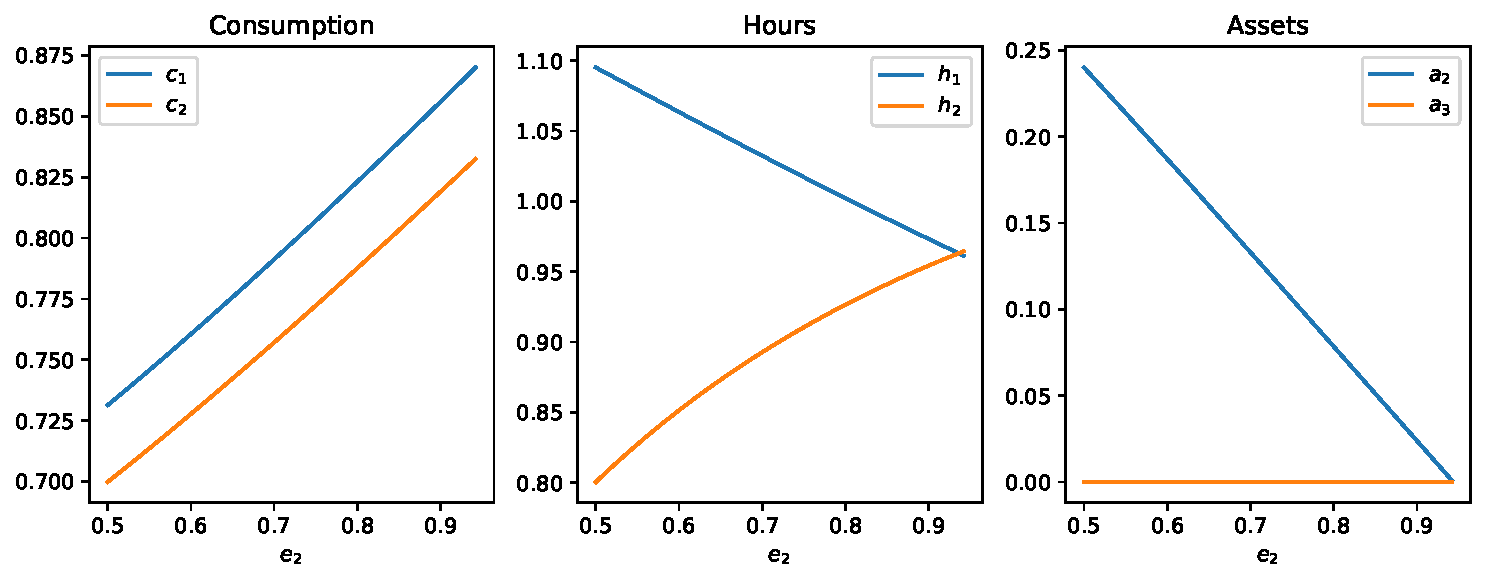
\includegraphics[width=\textwidth]{figures/problem4_policy_functions}
\caption{Period-1 policy functions as functions of $e_2$: consumption ($c_1$, $c_2$), hours ($h_1$, $h_2$), and assets ($a_2$, $a_3$). Plotted only where $a_2 > 0$ (interior). The second-period choices are evaluated at the endogenously chosen $a_2(e_2)$.}
\label{fig:problem4-policy}
\end{figure}

\clearpage
\section{Problem 5: Two-Period Portfolio Choice}

The consumer lives for two periods and has Epstein--Zin preferences
\begin{equation}
  V(m) =
  \left[
    c_1^{1-\gamma}
    + \beta
    \left(\E\, c_2^{1-\sigma}\right)^{\frac{1-\gamma}{1-\sigma}}
  \right]^{\frac{1}{1-\gamma}},
  \label{eq:p5-ez}
\end{equation}
where $\gamma$ is inverse EIS and $\sigma$ is risk aversion. The consumer begins period 1 with cash-on-hand $m>0$ and chooses (i) the savings share $x \ge 0$ and (ii) the risky share of savings $x_s \in [0,1]$ (no borrowing, no short-selling). Period-1 consumption is
\begin{equation}
  c_1 = (1-x)m.
\end{equation}
The consumer can invest savings $xm$ in a safe asset with gross return $R_f = 1+r$ or a risky asset with gross return $R = 1+r+\varepsilon_2$. Period-2 consumption is
\begin{equation}
  c_2 = y_2 + (1+r)xm + \varepsilon_2 x_s xm.
  \label{eq:p5-c2}
\end{equation}
The pair $(\log y_2,\varepsilon_2)$ is jointly normal:
\begin{equation}
  \begin{bmatrix}\log y_2 \\ \varepsilon_2\end{bmatrix}
  \sim \mathcal{N}\left(
  \begin{bmatrix}0 \\ \mu\end{bmatrix},
  \begin{bmatrix}
    \sigma_y^2 & \rho \sigma_y \sigma_\varepsilon \\
    \rho \sigma_y \sigma_\varepsilon & \sigma_\varepsilon^2
  \end{bmatrix}
  \right).
\end{equation}
We solve the problem for two correlations, $\rho \in \{0.3,0.6\}$.

\paragraph{Parameters.}
We use $\beta = 0.90$, $\sigma = 5$, $\gamma = 1/2$, $r = 0.04$, $\mu = 0.06$, $\sigma_\varepsilon = 0.15$, and $\sigma_y = 0.20$. We solve for a grid of cash-on-hand values $m \in [0.1,10]$.

\subsection{Optimality conditions and Euler equations}

Define the period-2 certainty equivalent
\begin{equation}
  CE_2 \equiv \left(\E\,c_2^{1-\sigma}\right)^{\frac{1}{1-\sigma}}.
\end{equation}
Since the outer power in \eqref{eq:p5-ez} is monotone, the choice problem is equivalent to maximizing
\begin{equation}
  J \equiv c_1^{1-\gamma} + \beta CE_2^{1-\gamma}.
\end{equation}
Let the stochastic discount factor associated with these preferences be
\begin{equation}
  M_2
  \equiv
  \left(\frac{c_2}{c_1}\right)^{-\gamma}
  \left(\frac{c_2}{CE_2}\right)^{\gamma-\sigma}.
  \label{eq:p5-sdf}
\end{equation}
At an interior optimum, the Euler equations for the safe and risky assets are
\begin{align}
\begin{split}
  1 &= \beta\,\E\left[ M_2 (1+r) \right],\\
  1 &= \beta\,\E\left[ M_2 (1+r+\varepsilon_2) \right].
\end{split}\label{eq:p5-euler}
\end{align}
These are the equations we use for diagnostic checks. When the constraints bind (e.g.\ $x=0$ or $x_s \in \{0,1\}$), the corresponding Euler equation need not hold with equality.

\subsection{Numerical solution}

\subsubsection{Quadrature for $(\log y_2,\varepsilon_2)$}

We approximate expectations with tensor-product Gauss--Hermite quadrature. This choice is natural because $(\log y_2,\varepsilon_2)$ is bivariate normal: Gauss--Hermite quadrature is designed for integrals with a Gaussian (normal) weight function, and the multivariate version uses a tensor product of one-dimensional Gauss--Hermite rules, matching the joint normal density.

The integrand $g(y_2,\varepsilon_2)$ in the quadrature is the object whose expectation we need. For the Euler equations \eqref{eq:p5-euler} this is the stochastic discount factor times the asset's gross return: $g = M_2 \times \text{(gross return)}$. The SDF $M_2$ depends on $(y_2,\varepsilon_2)$ through period-2 consumption $c_2 = y_2 + (1+r)xm + \varepsilon_2 x_s xm$. Concretely, for the safe-asset equation we use $g_{\text{safe}}(y_2,\varepsilon_2) = M_2(y_2,\varepsilon_2)\,(1+r)$; for the risky-asset equation we use $g_{\text{risky}}(y_2,\varepsilon_2) = M_2(y_2,\varepsilon_2)\,(1+r+\varepsilon_2)$. With nodes $\{(\log y_2^j,\varepsilon_2^j)\}_{j=1}^J$ and weights $\{w_j\}_{j=1}^J$ (with $\sum_j w_j=1$), we set $y_2^j = \exp(\log y_2^j)$ and approximate
\begin{equation}
  \E[g(y_2,\varepsilon_2)] \approx \sum_{j=1}^J w_j\, g(y_2^j,\varepsilon_2^j).
\end{equation}
We use $7$ nodes in each dimension (so $J=49$). 

\subsubsection{Optimization over $(x,x_s)$}

For each $m$ and each $\rho$, we solve the bounded two-dimensional maximization problem
\begin{equation}
  \max_{x\in[0,1],\,x_s\in[0,1]} \; V(m;x,x_s),
\end{equation}
where $V$ is defined by \eqref{eq:p5-ez}--\eqref{eq:p5-c2}. We solve via a bounded quasi-Newton optimizer (L-BFGS-B) on $-V$, using \texttt{hetmacro.optimize.minimize\_lbfgsb}.

\begin{algorithm}[H]
\caption{Solve policies for each $m$ and $\rho$}
\label{alg:p5-solve}
\begin{algorithmic}[1]
\State \textbf{Input:} $m$ grid, parameters $p$, correlation $\rho$
\State \textbf{Output:} policy functions $x(m)$ and $x_s(m)$
\State Build quadrature nodes/weights for $(\log y_2,\varepsilon_2)$
\For{each $m$}
  \State Solve $\max_{x,x_s\in[0,1]} V(m;x,x_s)$ via L-BFGS-B
\EndFor
\State \textbf{return} $x(m)$, $x_s(m)$
\end{algorithmic}
\end{algorithm}

\subsection{Results and Euler diagnostics}

\Cref{fig:p5-policies} plots the optimal saving share $x(m)$ and risky share $x_s(m)$ for $\rho=0.3$ and $\rho=0.6$. \Cref{fig:p5-euler} shows Euler residuals for the safe and risky asset, computed from \eqref{eq:p5-euler} and masked to points where both controls are interior (away from the bounds).

\begin{figure}[H]
\centering
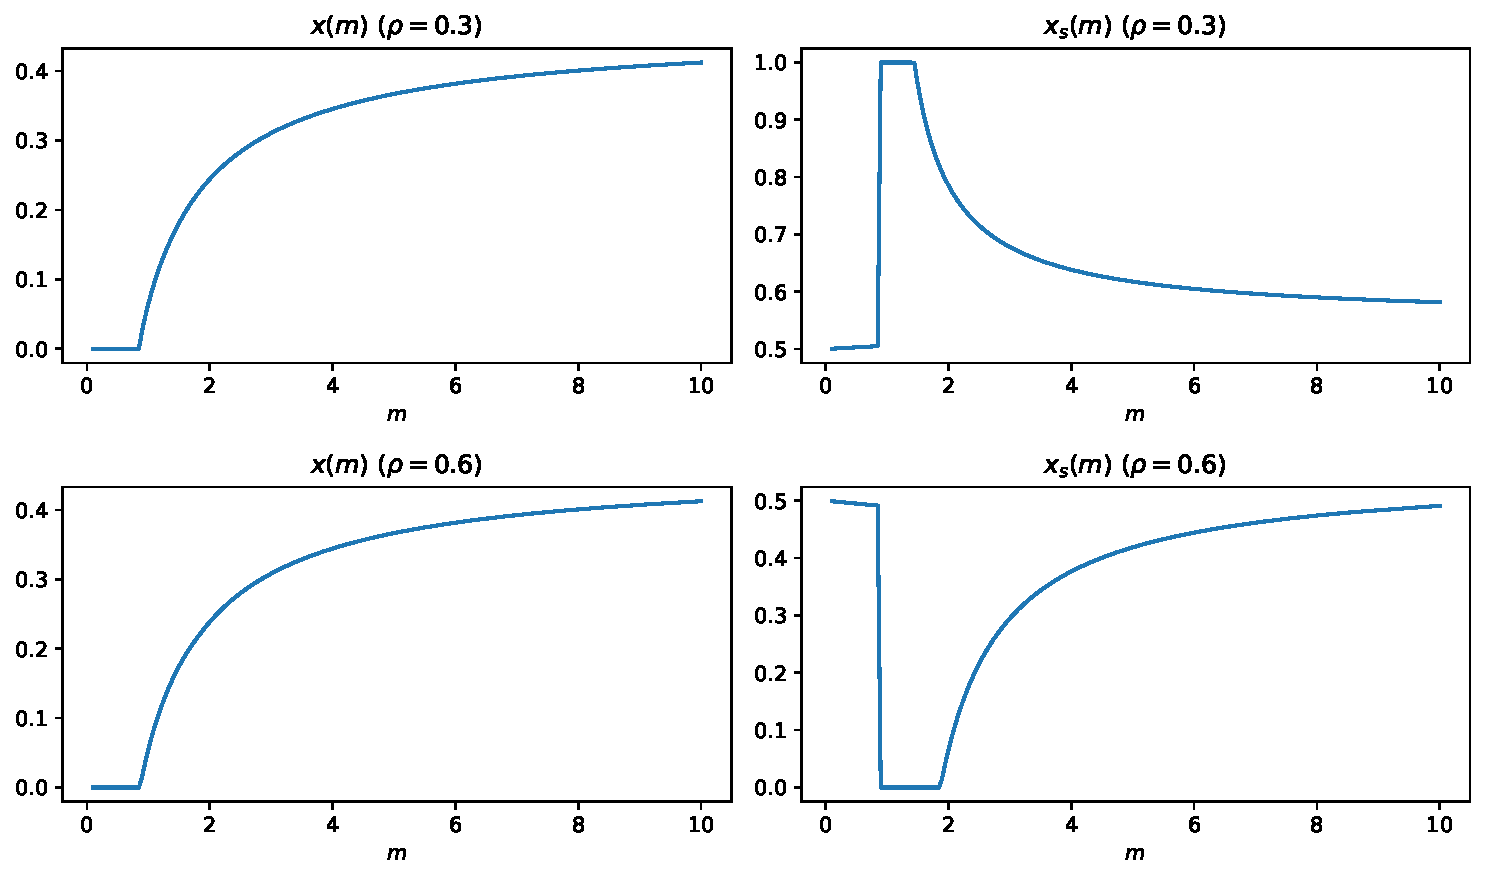
\includegraphics[width=0.95\textwidth]{figures/problem5_policies}
\caption{Problem 5 policy functions: saving share $x(m)$ and risky share $x_s(m)$ for correlations $\rho=0.3$ and $\rho=0.6$.}
\label{fig:p5-policies}
\end{figure}

\begin{figure}[H]
\centering
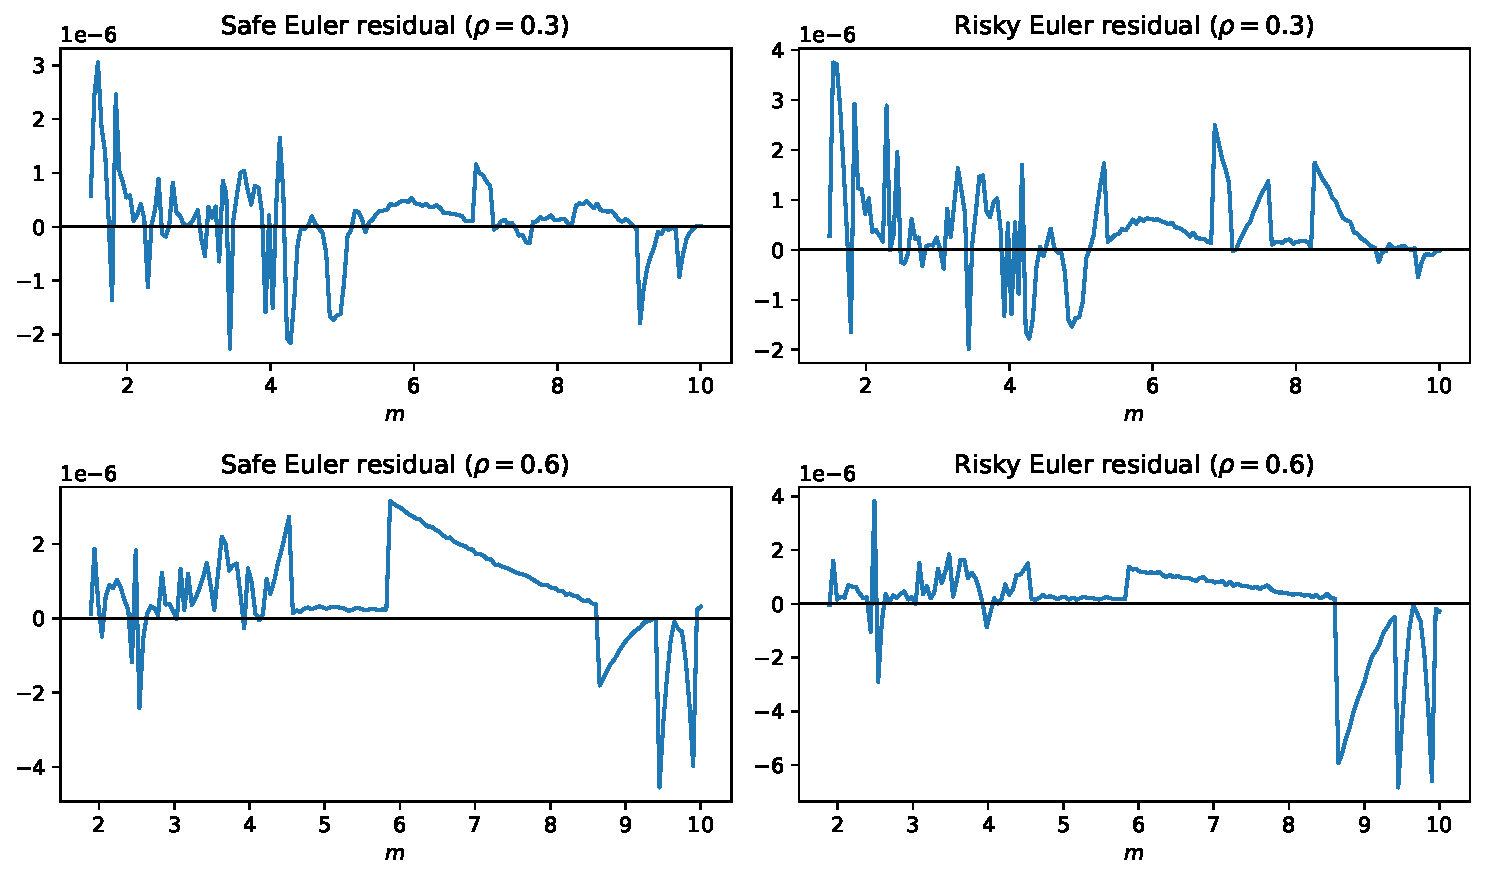
\includegraphics[width=0.95\textwidth]{figures/problem5_euler_residuals}
\caption{Euler residual diagnostics for the safe and risky asset, computed using the Epstein--Zin SDF \eqref{eq:p5-sdf} and masked to (approximate) interior points where $x\in(0,1)$ and $x_s\in(0,1)$.}
\label{fig:p5-euler}
\end{figure}



\end{onehalfspacing}
\end{document}

